\documentclass{beamer}

\usetheme[secheader]{Madrid}
\useinnertheme[]{rectangles}
\setbeamertemplate{navigation symbols}{}%remove navigation symbols


\usepackage[utf8]{inputenc}		% direct input of umlauts (other options: utf8, utf8x)
\usepackage[T1]{fontenc} 			% better c&p from pdf
\usepackage[english]{babel}		% language switch. use ngerman
\usepackage{csquotes}


%%%%%%%%%%%%%%%%%%%%%%%%%%%%%%%%%%%%%%%%%%%%%%%%%%%%%%%%%%%%%%%%
%%%%%%%%%%%%%%%%%%%%%%%%%%%  MATHS  %%%%%%%%%%%%%%%%%%%%%%%%%%%%
\usepackage{mathdots}	% inverse ddots \iddots
\usepackage{amsmath,amssymb,array}	% core math
\usepackage[centercolon]{mathtools}	% minor additions for ams
\usepackage{xfrac}	% 1/2 style fracs with \sfrac
\usepackage{cancel}	% cancel out terms


\usepackage{multicol}	% multicolumns environment
\usepackage{subcaption}	%subfigures

\usepackage{animate} %need the animate.sty file
\usepackage[backend=biber,style=authortitle]{biblatex}
\addbibresource{ad.bib}

%%%%%%%%%%%%%%%%%%%%%%%%%%%%%%%%%%%%%%%%%%%%%%%%%%%%%%%%%%%%%%%%
%%%%%%%%%%%%%%%%%%%%%%%%%%  FEATURES  %%%%%%%%%%%%%%%%%%%%%%%%%%

\usepackage[final]{listings}									% pretty print source code
	\lstloadlanguages{C++}
	\lstset{
		numbers=left, 
		numberstyle=\tiny, 
		basicstyle=\ttfamily,
		morecomment=[l][commentstyle]{//},
		commentstyle={\tiny\itshape},
		moredelim=**[is][\color{gray}]{@}{@},	% highlight between @..@
		aboveskip=\smallskipamount,
		belowskip=\smallskipamount,
		mathescape=true,
		breaklines,
	}
\newcommand{\src}[1]{\lstinline{#1}}
	
\usepackage{algorithm,algpseudocode}	% pseudo code

\usepackage{tikz,pgfplots}						% plotting
	
\usetikzlibrary{external}
\pgfkeys{/pgf/images/include external/.code=\includegraphics{#1}}	%draft mode for external tikz
\tikzsetexternalprefix{Bilder/tikz/}
\tikzexternalize

%%%%%%%%%%%%%%%%%%%%%%%%%%%%%%%%%%%%%%%%%%%%%%%%%%%%%%%%%%%%%%%%
%%%%%%%%%%%%%%%%%%%%%  Custom Commands  %%%%%%%%%%%%%%%%%%%%%%%%

\newcommand{\pma}[1]{\begin{pmatrix} #1 \end{pmatrix}}
\newcommand{\bma}[1]{\begin{bmatrix} #1 \end{bmatrix}}

\renewcommand{\d}{\mathchoice{\,d\!\;\!}{\,d}{\,d}{d}} %integral d

\DeclareMathOperator{\sgn}{sign}
\DeclareMathOperator{\diag}{diag}
\DeclareMathOperator{\abs}{abs}

\newcommand{\D}{\triangle}%%todo better symbol/space around
\newcommand{\pl}{\square}

\newcommand{\floor}[1]{\lfloor#1\rfloor}
\newcommand{\floorS}[1]{\left\lfloor#1\right\rfloor}
\newcommand{\ceil}[1]{\lceil#1\rceil}
\newcommand{\ceilS}[1]{\left\lceil#1\right\rceil}

\newcommand{\rx}{\mathring{x}}
\newcommand{\hx}{\hat{x}}
\newcommand{\cx}{\check{x}}


\title[Dataassimilation with PL]{Integrating and adjoining Lipschitzian ODEs with application to Dataassimilation}
\author[Lenser ]{Ben Lenser} 
\institute[]{

\includegraphics[height=0.3\textheight]{img/husiegel.pdf}\\[0.5cm]
Humboldt Universität zu Berlin\\Institut für Mathematik
}
\date{\today}

\begin{document}
\frame{\titlepage}
\frame{\tableofcontents}

%%%%%%%%%%%%%%%%%%%%%%%%%%%%%%%%%%%%%%%%%%%%%%%%%%%%%%%%%%%%%%%%
%%%%%%%%%%%%%%%%%%%%%%  CONTENTS  %%%%%%%%%%%%%%%%%%%%%%%%%%%%%%

%\include{richard.plain}
%\include{paul.plain}
\section[Datenassimilation]{4D- Datenassimilation}
\begin{frame}[<+->]
\frametitle{4D- Datenassimilation}
    \begin{itemize}
     \item Benutzt im Kontext der numerischen Wettervorhersage und ozeanographischen Modellen
     \item Eingeführt von Talagrand und Dimet $\approx$ 1986 (\cite{dimet1986variational})
     \item Ziel: Annäherung eines Modells an Observierungsparameter durch Steuerungsparameter um über $T$ hinaus zu extrapolieren
%      \item Wendet Methoden der optimalen Steuerung auf die Datenassimilation an
    \end{itemize}

\end{frame}

\begin{frame}
\frametitle{4D- Datenassimilation}
    \begin{block}{Voraussetzung}
    \parbox[c][3.5\baselineskip][t]{\textwidth}{
    \begin{itemize}
     \item $\dot{x} = F(x),~ x_0 = x(0),~F\in C^1(\R^n)$
%      \item $x_{obs}(t)$ - Observierungsparameter (Funktion oder diskrete Werte)
%      \item $C$ - Projektion von $X_{\text{State}}$ nach $X_{\text{Obs}}$ 
    \end{itemize}
    }
    \end{block}
   \begin{block}{Problem}
      \begin{tikzpicture}
     \begin{axis}[width=12cm,height=5cm,xlabel=t,ylabel=x] 
     \addplot[blue,domain=0:10,samples=100]{sin(deg(x))};
  \legend{$x$}
     \end{axis}
   \end{tikzpicture}
   \end{block}
\end{frame}
\begin{frame}
\frametitle{4D- Datenassimilation}
    \begin{block}{Voraussetzung}
    \parbox[c][3.5\baselineskip][t]{\textwidth}{
     \begin{itemize}
     \item $\dot{x} = F(x),~ x_0 = x(0),~F\in C^1(\R^n)$
     \item $x_{obs}(t)$ - Observierungsparameter (Funktion oder diskrete Werte)
%      \item $C$ - Projektion von $X_{\text{State}}$ nach $X_{\text{Obs}}$ 
    \end{itemize}
    } 
   \end{block}
   \begin{block}{Problem}
      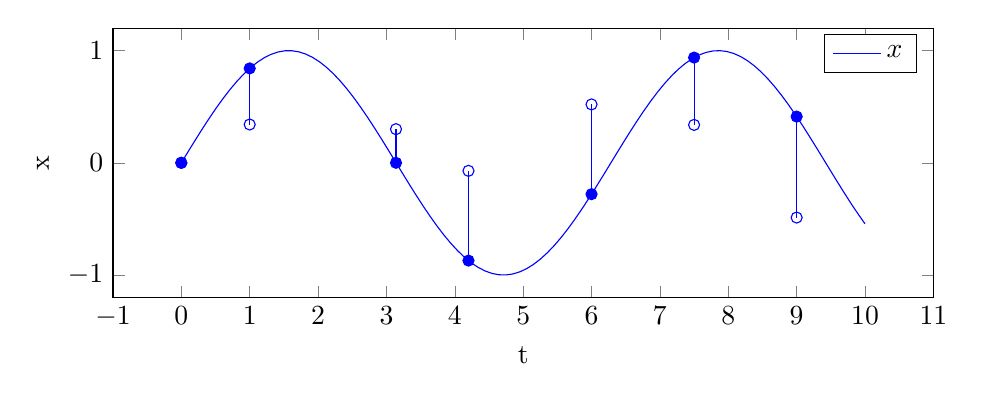
\begin{tikzpicture}
     \begin{axis}[width=12cm,height=5cm,xlabel=t,ylabel=x] 
     \addplot[blue,domain=0:10,samples=100]{sin(deg(x))};
     \addplot+[blue,draw=none,mark=*, mark options={blue},error bars/.cd, y dir=plus,y explicit,error mark=o,error mark options={blue,mark size=2pt}] 
     coordinates { 
      (0,0) +- (0,0) 
     (1,0.8415) +- (0.5,-0.5) 
     (3.14,0) +- (0.05,0.3) 
     (4.2,-0.8715) +- (0,0.8)
     (6.0,-0.27942) +- (0,0.8)
     (7.5,0.93799) +- (0.1,-0.6) 
     (9,0.41212) +- (0.3,-0.9)}; 
  \legend{$x$}
     \end{axis}
   \end{tikzpicture}
   \end{block}
\end{frame}



\begin{frame}[<+->]
  \frametitle{Datenassimilation Schritte}
	\begin{block}{Ziel: Minimiere Kostenfunktional}
	\begin{equation}\label{eq:costFunctional}
		\min_{x_o} J(x_0) = \min_{x_o} \frac{1}{2}\int_0^T \|Cx(t) - x_{Obs}(t)\|^2dt
	\end{equation}
	  $C$ - Projektion von $X_{\text{State}}$ nach $X_{\text{Obs}}$ 
	\end{block}
	\begin{block}{Datenassimilation Schritte}
	\begin{enumerate}
	 \item Berechnung Kostenfunktional
	 \item Berechnung $\nabla J(x_0)$
	 \item Optimierung
	\end{enumerate}
	\end{block}
\end{frame}
 
\begin{frame}[<+->]
  \frametitle{Datenassimilation Schritte}
  \begin{block}{Lösen einer ODE - z.B. Implizite Mittelpunktsregel(IMP)}
	\begin{equation}
	 x_n = x_a + h F \left(0.5 (x_a + x_n), t + 0.5 h\right)
	\end{equation}
	Speichere Werte $x_i$, berechne $J(x_0)$ mittels numerischer Quadratur
  \end{block}
  \begin{block}{Berechnung des Gradienten $\nabla J(x_0)$}
	Integriere das inhomogene adjungierte Tangent Linear Model rückwärts in $t$
	\begin{equation}
	  \dot{ \bar{x}}(t) =  -\frac{\partial F(x(t))}{\partial x}^\tr \bar x(t) +C^\tr(Cx(t) - x_{\text{obs}}(t)), ~ \bar x(T) =0
	\end{equation}
	\[
	\text{mit }\nabla J(x_0) = -\bar x(0)
	\]
  \end{block}
  \begin{block}{Optimierung}
	Optimiere $x_0$ mit einem geeigneten Verfahren über $J$ mit $\nabla J$ (z.B. BFGS)
  \end{block}

\end{frame} 

\begin{frame}[<+->]
  \frametitle{Problemstellung}
  \begin{block}{Problemstellung}
  \centering
	Wie kann die Datenassimilation für den Fall
	\[
	  \dot{x} = F(x),~ x_0 = x(0),~F\in C^{0,1}(\R^n)
	\]
	betrachtet werden?
  \end{block}
%   \begin{block}
   \begin{itemize}
    \item Unglatte Modelle in Ingeneursdisziplinen
    \item Elektrotechnik (Diode)
    \item Partielle Differentialgleichungen (Flux Limiter $\to$ Shallow Water Equation)
   \end{itemize}

%   \end{block}

\end{frame} 


\end{document}